\documentclass[]{article}
\usepackage{lmodern}
\usepackage{amssymb,amsmath}
\usepackage{ifxetex,ifluatex}
\usepackage{fixltx2e} % provides \textsubscript
\ifnum 0\ifxetex 1\fi\ifluatex 1\fi=0 % if pdftex
  \usepackage[T1]{fontenc}
  \usepackage[utf8]{inputenc}
  \usepackage{eurosym}
\else % if luatex or xelatex
  \ifxetex
    \usepackage{mathspec}
  \else
    \usepackage{fontspec}
  \fi
  \defaultfontfeatures{Ligatures=TeX,Scale=MatchLowercase}
  \newcommand{\euro}{€}
\fi
% use upquote if available, for straight quotes in verbatim environments
\IfFileExists{upquote.sty}{\usepackage{upquote}}{}
% use microtype if available
\IfFileExists{microtype.sty}{%
\usepackage[]{microtype}
\UseMicrotypeSet[protrusion]{basicmath} % disable protrusion for tt fonts
}{}
\PassOptionsToPackage{hyphens}{url} % url is loaded by hyperref
\usepackage[unicode=true]{hyperref}
\hypersetup{
            pdfborder={0 0 0},
            breaklinks=true}
\urlstyle{same}  % don't use monospace font for urls
\usepackage{graphicx,grffile}
\makeatletter
\def\maxwidth{\ifdim\Gin@nat@width>\linewidth\linewidth\else\Gin@nat@width\fi}
\def\maxheight{\ifdim\Gin@nat@height>\textheight\textheight\else\Gin@nat@height\fi}
\makeatother
% Scale images if necessary, so that they will not overflow the page
% margins by default, and it is still possible to overwrite the defaults
% using explicit options in \includegraphics[width, height, ...]{}
\setkeys{Gin}{width=\maxwidth,height=\maxheight,keepaspectratio}
\IfFileExists{parskip.sty}{%
\usepackage{parskip}
}{% else
\setlength{\parindent}{0pt}
\setlength{\parskip}{6pt plus 2pt minus 1pt}
}
\setlength{\emergencystretch}{3em}  % prevent overfull lines
\providecommand{\tightlist}{%
  \setlength{\itemsep}{0pt}\setlength{\parskip}{0pt}}
\setcounter{secnumdepth}{0}
% Redefines (sub)paragraphs to behave more like sections
\ifx\paragraph\undefined\else
\let\oldparagraph\paragraph
\renewcommand{\paragraph}[1]{\oldparagraph{#1}\mbox{}}
\fi
\ifx\subparagraph\undefined\else
\let\oldsubparagraph\subparagraph
\renewcommand{\subparagraph}[1]{\oldsubparagraph{#1}\mbox{}}
\fi

% set default figure placement to htbp
\makeatletter
\def\fps@figure{htbp}
\makeatother


\date{}

\begin{document}

\section{Kafka: streaming data}\label{kafka-streaming-data}

\subsection{Indice}\label{indice}

\begin{enumerate}
\def\labelenumi{\arabic{enumi}.}
\tightlist
\item
  \protect\hyperlink{motivazioni}{Motivazioni}\\
\item
  \protect\hyperlink{introduzione}{Introduzione}\\
  2.1. \protect\hyperlink{etl}{ETL}\\
  2.2. \protect\hyperlink{intro-data}{L'importanza dei dati e degli
  eventi}\\
  2.3. \protect\hyperlink{event-sourcing}{Event sourcing}\\
  2.4. {[}Stream processing{]}\\
  2.5. {[}Svantaggi di un processo ETL: confronto ETL \textasciitilde{}
  ES+Stream processing{]}
\item
  {[}Apache Kafka e l'ecosistema{]}\\
  3.1. {[}Struttura generica di Kafka{]}\\
  3.2. {[}Kafka Connect{]}\\
  3.3. {[}Kafka Streams{]}\\
\item
  {[}Esempi di utilizzo{]}\\
\item
  {[}Bibliografia{]} \newpage
\end{enumerate}

\hypertarget{motivazioni}{\subsection{1.
Motivazioni}\label{motivazioni}}

Negli ultimi anni l'avvento delle architetture a microservizi ha portato
la necessità di studiare nuove soluzioni al problema della gestione di
molteplici fonti di dati.

In sistemi complessi formati da più microservizi tanti componenti
interdipendenti comunicano tra loro scambiandosi dati e attingendo da
numerose fonti di dati comuni come database, data warehouses oppure
servizi esterni.

La necessità di filtrare, standardizzare e gestire molte fonti di dati
aveva portato alla nascita del processo di \textbf{Extract, Transform,
Load} (ETL) per l'estrazione, trasformazione e caricamento di dati in
sistemi di sintesi come data warehouse o data mart, questo processo si
sta però rivelando complicato ed impegnativo in un mondo dove la mole di
dati prodotta dal logging di eventi critici ad un qualsiasi business è
in continua crescita: semplici esempi sono la gestione degli eventi in
un sistema \textbf{Internet of things} (IoT) oppure lo studio delle
abitudini dei propri clienti per un servizio di e-commerce.

Lo stream processing tra microservizi propone un nuovo approccio per la
gestione di questi problemi, fornendo una soluzione adatta alla gestione
di dati in real-time altamente scalabile e ad alto throughput.

Apache Kafka è una piattaforma nata in un contesto aziendale importante
che mira a rivoluzionare il modo con cui i microservizi di un business
comunicano tra loro, favorendo un approccio improntato sulla gestione di
eventi legati al comportamento dei dati, più che i dati in se.\\
Kafka nasce per sfruttare a pieno lo stream processing e favorire una
gestione intelligente di grosse moli di dati, abbandonando il classico
processo ``batch'' ETL per una soluzione, appunto, basata sullo
streaming dei dati tra microservizi.

\newpage

\hypertarget{introduzione}{\subsection{2.
Introduzione}\label{introduzione}}

Prima di poter discutere della architettura fornita da Apache Kafka, è
necessario comprendere le differenze tra ETL e stream processing.\\
Per poter utilizzare pienamente stream processing, è inoltre necessario
comprendere come la gestione di dati basata su inserimento,
cancellazione e modifica da database, può essere modellata come una
serie di eventi e quali sono i vantaggi di un approccio alla gestione di
questi dati basato su \textbf{event sourcing} (ES).

\hypertarget{etl}{\subsubsection{2.1 ETL}\label{etl}}

\begin{quote}
Cos'è un processo di etl
\end{quote}

Un processo di Extract, Transform, Load (ETL) è un processo mirato alla
trasformazione di dati contenuti su più database per ottenere un nuovo
insieme di dati, filtrato e traformato secondo una particolare logica,
destinato ad essere salvato in una data warehouse.\\
Verso la fine degli anni '70 molte aziende iniziarono ad utilizzare
molteplici database per salvare e gestire informazioni, è proprio in
questo contesto che nascono i processi di ETL: con l'avanzare del tempo
è stato necessario studiare un metodo per l'aggregazione e gestione
delle varie fonti di dati.

Un qualsiasi processo di ETL si compone di tre parti:

\begin{quote}
Extract
\end{quote}

E' la prima parte del processo di ETL ed involve l'estrazione dei dati
da più data sources come database relazionali o non-relazionali, file
JSON od XML ma anche risorse ``adhoc'' come, ad esempio, dei dati
generati da programmi di web analytics.

L'obiettivo di questa fase è estrarre tutti i dati necessari dalle
possibili sorgenti e prepararli alla fase di Transform.

Un importante problema legato a questa fase è il processo di
\textbf{validazione delle sorgenti dati}: con più sorgenti dati spesso
ci si ritrova a dover gestire più \emph{formati} non necessariamente
compatibili tra loro.\\
Per poter garantire alla fase di Transform dei dati comprensibili,
durante la fase di Extract vengono definite delle \emph{regole di
validazione} per filtrare i dati provenienti dalle varie sorgenti, un
esempio di regola di validazione è il controllo dei tipi di dati
presenti nella fonte.

\begin{quote}
Transform
\end{quote}

Nella fase di Transform una serie di regole e funzioni vengono applicate
ai dati generati dalla fase di Extract per prepararli alla fase di Load
nella data warehouse.

Il primo compito della fase di Transform è la \textbf{pulizia dei dati}:
spesso le varie fonti di dati, nonostante siano state validate, possono
presentare incongruenze tra loro come caratteri speciali legati
all'encoding della propria sorgente oppure formati dei dati diversi ma
compatibili (un esempio può essere la differneza di formattazione tra
date americane ed europee).\\
Per garantire un corretto funzionamento delle operazioni di
trasformazione è quindi necessario pulire i dati ed adattarli ad un
formato comune.

Il secondo compito della fase di Transform è la \textbf{trasformazione
dei dati} in nuovi dati richiesti dal business, esempi di trasformazioni
sono:

\begin{itemize}
\tightlist
\item
  Joining di tabelle da più sorgenti
\item
  Mapping e trasformazione di dati (esempio: ``Maschio'' in ``M'')
\item
  Aggregazione di dati
\item
  Generazione/calcolo di nuovi dati
\item
  Selezione di insiemi di dati
\item
  Validazione del nuovo formato di dati prodotto
\end{itemize}

\begin{quote}
Load
\end{quote}

Nella fase di Load l'insieme di dati generati dalla fase di Transform
vengono inseriti in un target, il quale potrebbe essere una data
warehouse ma anche più semplicemente un file in un formato utile.\\
Business diversi hanno necessità diverse, per questo l'implementazione
della fase di load può avere più modalità implementative, il punto
focale di questa fase è proprio stabilire la frequenza e le modalità di
aggiornamento dei dati presenti nel target.\\
Decidere la frequenza (giornaliera, mensile, ecc.) e le modalità
(sovrascrizione dei vecchi dati o meno) del target possono portare ad un
processo di ETL più o meno utile ad una azienda.

Per generare un buon target è buona norma definire uno schema
\emph{preciso e chiaro} della tipologia di dati a cui il target deve
aderire.\\
Come detto in precedenza un processo di ETL è utilizzato per aggregare
più fonti di informazioni comuni ad un processo aziendale, questo
suppone che le informazioni presenti nella data warehouse potrebbero
venire usate da più parti di una azienda, le quali potrebbero essere
abituate a particolari formati dei dati.\\
Senza definire uno schema dei dati chiaro e preciso, si correrebbe il
rischio di generare un insieme di dati inutilizzabile da determinati
reparti in quanto non conforme al formato di dati da loro conosciuto.

\newpage

\subsubsection{2.2 L'importanza dei dati e degli eventi \{piccola
introduzione per
ES\}}\label{limportanza-dei-dati-e-degli-eventi-piccola-introduzione-per-es}

Lo status quo delle moderne applicazioni web è basato sul utilizzo di
database per rappresentare le specifiche di dominio, spesso espresse da
un cliente e/o da un esperto del dominio esterno all'ambiente di
sviluppo.

Durante la fase di analisi dei requisiti (supponendo un modello di
sviluppo del software agile) cliente e team di sviluppo si confrontano,
cercando di trovare un linguaggio comune per definire la logica e
l'utilizzo del software richiesto; Una volta stabiliti i requisti, il
team di sviluppo generalmente inizia uno studio interno atto a produrre
un \textbf{modello dei dati} che verrà usato come base per definire lo
schema dei database utilizzati dal sistema.\\
Un cliente comune molto spesso non ha padronanza del concetto di `stato
di una applicazione', ma piuttosto si limita ad esporre i propri
requisiti descrivendo i possibili \textbf{eventi} che, traslati sul
modello di sviluppo incentrato su i database, portano il team di
sviluppo a ragionare sui possibili stati di un database in risposta a
questi eventi.

Lo stato di un database di una applicazione è strettamente legato
all'insieme degli eventi del dominio applicativo; L'unico modo per
modificare o interagire con questo database è tramite i comandi di
inserimento, cancellazione o lettura, tutti comandi che vengono eseguiti
solamente all'avvenire di un particolare evento.

Un database mantiene solo lo stato corrente di una applicazione; Non
esiste il concetto di cronologia del database a meno di utilizzare
soluzioni basate su \textbf{Change Data Capture} (CDC), generalmente
utilizzate per generare un transactional log contenente tutte le
operazioni eseguite sul suddetto database.\\
In questo modello database-driven, un evento genera un cambiamento su
una base di dati; Gli eventi e lo stato di un database sono però
concetti diversi e slegati tra loro, l'esecuzione di un evento a volte
può portare ad una asincronia tra l'esecuzione di un evento e lo stato
di un database, tanto più se questo database è utilizzato da tutti i
microservizi di una applicazione.

Una soluzione al problema di più microservizi che utilizzano lo stesso
database è di utilizzare delle views del database locali ad ogni
microservizio: ogni servizio lavorerà su una copia locale del database
ed un job esterno si occuperà di compattare le views e mantenere il
database aggiornato rispetto a tutti i cambiamenti.\\
Questa soluzione ha un enorme problema: supponiamo di notare un errore
sul database e di doverlo correggere, come possiamo decidere quale delle
views è ``più corretta'' delle altre? Per aiutarci nella ricerca
dell'errore potremmo utilizzare il transactional log di ogni views, ma
su database di grandezze importanti potrebbe essere un problema non
indifferente.

Event sourcing propone di risolvere questo genere di problemi
allontanandosi da una progettazione database-driven e basata sul pattern
di richiesta/risposta a risorse elevando gli eventi a elementi chiavi
del modello dei dati di una applicazione.

\newpage

\hypertarget{event-sourcing}{\subsubsection{2.3. Event
sourcing}\label{event-sourcing}}

\begin{quote}
Event Sourcing ensures that all changes to application state are stored
as a sequence of events. Not just can we query these events, we can also
use the event log to reconstruct past states, and as a foundation to
automatically adjust the state to cope with retroactive changes.
\end{quote}

Event sourcing (ES) è un design pattern che si contrappone ad una
visione del mondo\^{} basata su tabelle e schemi di uno o più database.

Durante l'analisi dei requisiti di una applicazione, spesso ci si trova
a confronto con esperti di un dominio applicativo che non hanno
particolare conoscenza delle tecnologie necessarie per implementare le
loro richieste, è compito del programmatore (o del team di
programmatore) analizzare le sue richieste e trasformarle in idee
gestibili.\\
In genere questi esperti spiegheranno al programmatore le loro necessità
illustrando il funzionamento del dominio utilizzando concetti molto più
vicini a degli \emph{eventi} piuttosto che \emph{sequenze di
richieste/risposte a/da un database}.

Supponiamo di dover sviluppare una soluzione software per una
piattaforma di e-commerce, avremo tre microservizi:

\begin{itemize}
\tightlist
\item
  UI / frontend
\item
  Servizio per la gestione degli ordini
\item
  Servizio stock
\end{itemize}

\begin{figure}
\centering
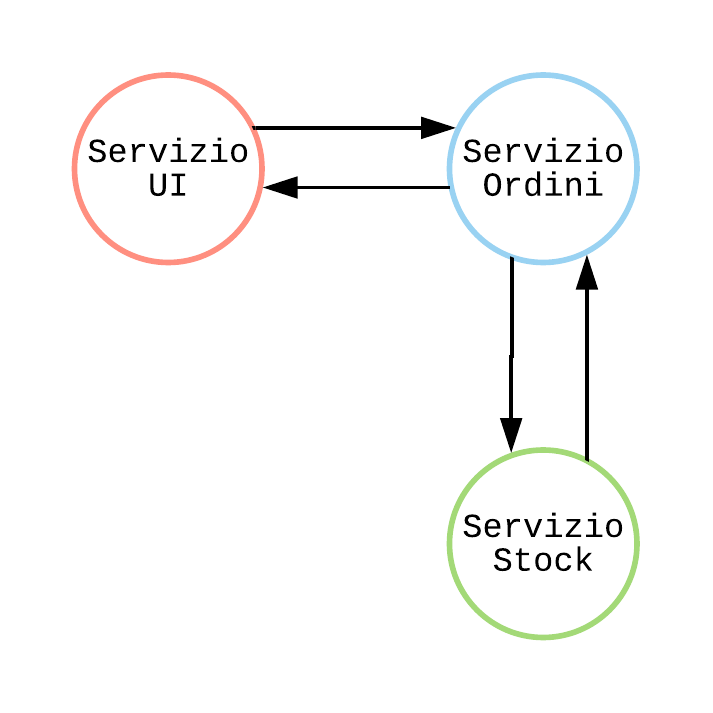
\includegraphics[width=0.50000\textwidth]{../images/figure1.png}
\caption{Esempio setup \label{my_label}}
\end{figure}

{[}\ldots{}{]}

Event sourcing (ES) è un design pattern basato su due fondamenti:

\begin{itemize}
\tightlist
\item
  Ogni cambiamento di stato del mondo è da vedersi come un evento; Ogni
  evento deve essere salvato
\item
  Tutti gli eventi devono essere salvati in sequenza, seguendo l'ordine
  in cui sono avvenuti
\end{itemize}

{[}\ldots{}{]}

\begin{quote}
Esempio di utilizzo di event sourcing =\textgreater{} come faccio? è
giusto copiare l'esempio che c'è già su un sito in modo da sfruttarne le
figure?
\end{quote}

\begin{quote}
Problemi risolti da event sourcing =\textgreater{} ho un log di
cambiamenti, semplicità nella gestione dei cambiamenti
\end{quote}

\begin{quote}
Problemi creati da event sourcing\\
=\textgreater{} può essere complicato eseguire query del tipo ``voglio
tutti gli ordini con valore \textgreater{}50\euro{}'' in quanto richiede
la generazione dello stato corrente del mondo, ovvero la lettura ed
esecuzione di tutto il log\\
-\textgreater{} risolvibile creando views parallele al log
\end{quote}

\subsubsection{2.4 Stream Processing}\label{stream-processing}

\begin{quote}
Descrivere le caratteristiche principali di un sistema di streaming :
distribuito, append only, etc.
\end{quote}

\begin{quote}
Differenza tra Message Brokers e transactional append only logs: Rabbit
MQ vs Kafka
\end{quote}

\subsubsection{2.5. Svantaggi di un processo ETL: perchè favorire stream
processing ed event
sourcing}\label{svantaggi-di-un-processo-etl-perchuxe8-favorire-stream-processing-ed-event-sourcing}

\begin{quote}
Introdurre il concetto di schema
\end{quote}

\begin{quote}
Perchè la gestione dei dati è importante nelle architetture a
microservizi
\end{quote}

\subsection{3. Apache Kafka e
l'ecosistema}\label{apache-kafka-e-lecosistema}

\subsubsection{3.1 Descrizione generica
Kafka}\label{descrizione-generica-kafka}

\begin{quote}
Struttura di base: log =\textgreater{} log compaction
\end{quote}

\begin{quote}
Struttura architetturale: * brokers * clusters * topic
\end{quote}

\begin{quote}
Come collegare event sourcing e kafka =\textgreater{} perchè kafka è una
buona piattaforma per event sourcing
\end{quote}

\subsubsection{3.2 Kafka Connect}\label{kafka-connect}

\begin{quote}
Schema
\end{quote}

\begin{quote}
Source connectors
\end{quote}

\begin{quote}
Sink connectors
\end{quote}

\begin{quote}
Community involment
\end{quote}

\subsubsection{3.3 Kafka Streams}\label{kafka-streams}

\begin{quote}
cos'è streams
\end{quote}

\begin{quote}
KSQL/LSQL
\end{quote}

\subsection{4. Esempi di utilizzo di
Kafka}\label{esempi-di-utilizzo-di-kafka}

\newpage

\subsection{5. Bibliografia}\label{bibliografia}

https://martinfowler.com/eaaDev/EventSourcing.html\\
https://www.confluent.io/blog/data-dichotomy-rethinking-the-way-we-treat-data-and-services/\\
https://www.confluent.io/blog/build-services-backbone-events/\\
https://www.confluent.io/blog/apache-kafka-for-service-architectures/\\
https://www.confluent.io/blog/messaging-single-source-truth/\\
https://www.confluent.io/blog/building-a-microservices-ecosystem-with-kafka-streams-and-ksql/\\
https://content.pivotal.io/blog/understanding-when-to-use-rabbitmq-or-apache-kafka\\
https://qconsf.com/sf2016/system/files/keynotes-slides/etl\_is\_dead\_long-live\_streams.pdf
\textless{}= https://www.youtube.com/watch?v=I32hmY4diFY

\end{document}
